\documentclass[conference]{IEEEtran}
\IEEEoverridecommandlockouts
\usepackage[T1]{fontenc}
\usepackage{cite}
\usepackage{amsmath,amssymb}
\usepackage{graphicx}
\usepackage{booktabs}
\usepackage{multirow}
\usepackage{xcolor}
\usepackage{algorithm}
\usepackage{algpseudocode}
\usepackage{tikz}
\usetikzlibrary{positioning,arrows.meta,fit,calc}
\usepackage[hidelinks]{hyperref}
\usepackage{url}

\newcommand{\repo}{\url{https://github.com/UsmanBari/trial-eligibility-transformer}}
\newcommand{\videolink}{\url{https://youtu.be/yTGi0hUCeyk}}

\begin{document}

\title{Evidence-Grounded Criterion-Level Clinical Trial\\Eligibility Screening with a LoRA-Tuned Small\\Decoder and Hand-Built Inference Mechanisms}

\author{\IEEEauthorblockN{Usman Bari (23i-0680)}
\IEEEauthorblockA{Department of Computer Science, FAST-NUCES Islamabad, Pakistan\\
i230680@isb.nu.edu.pk\\
Generative AI (AI-4009), Assignment 2}}

\maketitle

\begin{abstract}
Matching a patient to a clinical trial requires checking every inclusion and exclusion criterion against an unstructured clinical note and pointing to the sentences that justify each decision. We fine-tune Qwen2.5-1.5B-Instruct with Low-Rank Adaptation (LoRA) on the TrialGPT Criterion Annotations dataset, using the prescribed patient-grouped 37/8/8 split, so that it returns one of the dataset's six expert labels together with the supporting sentence IDs as JSON. A class-balanced variant, selected on validation data only, raises held-out test macro-F1 from 0.156 (zero-shot) to 0.632 and accuracy from 0.170 to 0.718, with evidence micro-F1 rising from 0.206 to 0.575. Around the model we implement, from first principles, (i)~a KV-cached greedy decoder that is token-identical to a no-cache reference on all 20 task prompts and up to 6.9$\times$ faster, (ii)~a tiled online-softmax attention that matches reference attention on 72/72 test configurations and uses 54$\times$ less memory at 8\,192 tokens, and (iii)~greedy speculative decoding with a 0.5B draft model and a prompt-lookup drafter. All speculative outputs equal plain greedy decoding; the draft model is slower because one draft step costs 0.84--0.89 of a target step, which a measured cost model predicts, whereas prompt lookup is 1.16--2.00$\times$ faster on a T4 GPU. A browser application exposes the screening workflow, evidence highlighting, report export and a live decoder comparison.
\end{abstract}

\begin{IEEEkeywords}
clinical trial matching, large language models, LoRA, KV cache, FlashAttention, speculative decoding, evidence retrieval
\end{IEEEkeywords}

% ======================================================================
\section{Introduction}
Recruiting patients is a major bottleneck of clinical research. A coordinator has to read a patient's history and decide, for each eligibility criterion of a trial, whether the patient satisfies it, violates it, whether it does not apply, or whether the record simply does not say. Large language models (LLMs) can automate part of this reading, but a usable screener must (a)~keep the ``not enough information'' and ``not applicable'' outcomes instead of forcing a yes/no answer, (b)~cite the exact patient sentences behind every decision so that a human can verify it, and (c)~run on hardware that a hospital or a student actually has.

\textbf{Problem statement.} Given a patient note split into numbered sentences, a criterion type (inclusion or exclusion) and the criterion text, predict the expert eligibility label and the set of supporting sentence IDs. The common benchmark is the TrialGPT Criterion Annotations dataset~\cite{jin2024trialgpt} evaluated on a fixed patient-grouped split.

\textbf{Contributions.}
\begin{enumerate}
\item A reproducible data pipeline with the prescribed 37/8/8 split, published manifest, leakage assertions, removal of all GPT-4 columns and a guarded, logged test split.
\item A LoRA-tuned Qwen2.5-1.5B screener with completion-only supervised fine-tuning, validation-based checkpoint and recipe selection, and a class-balanced variant that fixes the minority-class collapse of the first model.
\item Hand-written KV-cached decoding (with prefix reuse across criteria), tiled online-softmax attention that runs inside the full model, and greedy speculative decoding with explicit cache rollback, each validated for exactness and benchmarked with synchronised repeated timing.
\item A browser application with evidence highlighting, a rule-based overall verdict, report export and a live inference comparison.
\end{enumerate}

% ======================================================================
\section{Related Work}
\textbf{Patient--trial matching.} Koopman and Zuccon released a test collection pairing patient case reports with trials~\cite{koopman2016test}; its patients are the ones annotated here. TrialGPT~\cite{jin2024trialgpt} prompts GPT-4 to judge each criterion and cite sentences, and released the expert criterion-level annotations that we use. TrialGPT relies on a proprietary API; our system instead adapts a small open-weight model that runs locally, at the cost of a weaker base model. The GPT-4 predictions shipped with the dataset are never used as inputs or targets.

\textbf{Small decoders and adaptation.} The Transformer~\cite{vaswani2017attention} with rotary position embeddings (RoPE)~\cite{su2024roformer} and grouped-query attention (GQA)~\cite{ainslie2023gqa} is the standard modern decoder. Qwen2.5~\cite{qwen2025report} and SmolLM2~\cite{allal2025smollm2} provide open 0.5--1.7B checkpoints. Full fine-tuning of such a model does not fit a 16\,GB T4; LoRA~\cite{hu2022lora} freezes the weights and trains low-rank updates, which reduces optimiser memory by orders of magnitude and produces small, shareable adapters.

\textbf{Efficient inference.} Autoregressive decoding at batch size one is memory-bandwidth bound; caching keys and values avoids recomputing the prefix at every step~\cite{pope2023efficiently}, and GQA shrinks that cache. Prefix sharing, as in PagedAttention~\cite{kwon2023paged}, reuses the cache of a common prompt prefix. FlashAttention~\cite{dao2022flashattention} computes exact attention in tiles using the online softmax normaliser of Milakov and Gimelshein~\cite{milakov2018online}, so the $L\times L$ score matrix is never stored. Speculative decoding~\cite{leviathan2023fast,chen2023accelerating} lets a cheap drafter propose $k$ tokens that the target verifies in one pass; it is lossless, but its speedup depends on the draft cost and acceptance rate. Prompt-lookup decoding~\cite{saxena2023prompt} replaces the draft model with $n$-gram copying from the prompt.

\textbf{Limitations of the alternatives.} A proprietary LLM gives the best zero-shot accuracy but cannot be fine-tuned, inspected or run offline. Larger open models (7B+) need quantisation to fit our hardware and are slow on a laptop CPU. Fused attention kernels are fast but hide the algorithm, which is why we implement the tiled computation ourselves and compare against the fused kernel only as a reference.

% ======================================================================
\section{Materials and Methods}

\subsection{Dataset and fixed split}
The dataset has 1\,015 criterion annotations for 53 patients and 103 trials, each with the patient note, criterion type and text, an expert label, and expert evidence sentence IDs. We drop \texttt{gpt4\_explanation}, \texttt{gpt4\_sentences}, \texttt{gpt4\_eligibility}, \texttt{explanation\_correctness} and the original \texttt{training} flag before any processing. Unique patient IDs are sorted, shuffled with \texttt{numpy.random.default\_rng(42)}, and assigned 37/8/8 to train/validation/test. Hard assertions check that no patient, and no identical note text, appears in two splits and that every annotation is assigned exactly once; one row with an empty criterion is dropped. Table~\ref{tab:split} summarises the split. The label distribution is highly skewed: ``not excluded'' and ``not enough information'' dominate, the test split contains no gold ``excluded'' label, and 70\% of test criteria have no annotated evidence. The evaluation script refuses the test split unless an explicit \texttt{--final-test} flag is given and appends every test access to a log, so the test set was only used for the final comparisons reported in Section~\ref{sec:results}.

\begin{table}[t]
\centering
\caption{Patient-grouped split (seed 42) and label counts.}
\label{tab:split}
\footnotesize
\setlength{\tabcolsep}{3.5pt}
\begin{tabular}{lrrr}
\toprule
 & Train & Val & Test \\
\midrule
Patients & 37 & 8 & 8 \\
Criteria (incl./excl.) & 602 (215/387) & 206 (66/140) & 206 (75/131) \\
No gold evidence & 348 & 116 & 145 \\
\midrule
included & 88 & 35 & 27 \\
not included & 13 & 3 & 7 \\
excluded & 8 & 2 & 0 \\
not excluded & 291 & 101 & 91 \\
not enough information & 174 & 53 & 66 \\
not applicable & 28 & 12 & 15 \\
\bottomrule
\end{tabular}
\end{table}

\subsection{Input and output format}
Notes in the dataset are numbered ``\texttt{0.} \dots\ \texttt{1.} \dots''. We split them by scanning only for the next expected number at a line or whitespace boundary, so numbers inside sentences (doses, ``2. children'') do not create false boundaries and the IDs remain the ones the experts used. The user message contains the numbered sentences as \texttt{[i] text}, the criterion type, the criterion text, and the four labels allowed for that type with one-line definitions. The target is a single line of JSON, \texttt{\{"label": "\dots", "evidence": [ids]\}}, rendered with the Qwen chat template. Labels are kept exactly as in the dataset (four per criterion type, six in total). A label that is not allowed for the criterion type, or unparseable output, is scored as \emph{invalid} and counted as wrong rather than silently remapped; cited IDs that do not exist in the note are removed and logged. The explanation shown to users is built deterministically from the predicted label and the cited sentences, so it only quotes the record.

\textbf{Truncation.} The prompt budget is 3\,072 tokens; if exceeded, whole sentences are removed from the end of the note and the removed IDs, and any gold evidence among them, are logged. The longest prompt was 667 tokens in training and 544 in test, so no example was truncated and no evidence was lost.

\subsection{Model selection}
Table~\ref{tab:models} compares the candidates. Both 1.5--1.7B models fit a free 16\,GB T4 in fp16 with room for LoRA training, and both are Apache-2.0. We chose Qwen2.5-1.5B-Instruct because (i)~GQA with two KV heads makes its cache 6.9$\times$ smaller per token than SmolLM2's full multi-head attention, which matters for the KV and speculative experiments; (ii)~it has a 32K context against 8K; (iii)~a 0.5B sibling with the identical tokenizer exists, which speculative decoding requires; and (iv)~zero-shot, both models were equally weak at classification, but Qwen's evidence micro-F1 was twice SmolLM2's (Table~\ref{tab:models}). Qwen2.5-3B was rejected: its weights alone take 6\,GB in fp16, roughly doubling training time on the T4, and the application would need about 12\,GB of RAM on the author's 16\,GB laptop.

\begin{table}[t]
\centering
\caption{Decoder candidates (zero-shot scores on validation).}
\label{tab:models}
\footnotesize
\setlength{\tabcolsep}{2.5pt}
\begin{tabular}{lccc}
\toprule
 & \textbf{Qwen2.5-1.5B} & SmolLM2-1.7B & Qwen2.5-0.5B \\
 & (target) & (rejected) & (draft) \\
\midrule
Parameters & 1.54B & 1.71B & 0.49B \\
Layers / hidden & 28 / 1536 & 24 / 2048 & 24 / 896 \\
Q / KV heads & 12 / 2 (GQA) & 32 / 32 & 14 / 2 (GQA) \\
Vocabulary & 151\,936 & 49\,152 & 151\,936 \\
Context & 32\,768 & 8\,192 & 32\,768 \\
Licence & Apache-2.0 & Apache-2.0 & Apache-2.0 \\
fp16 weights & 3.1\,GB & 3.4\,GB & 1.0\,GB \\
KV cache / token & 28\,KB & 192\,KB & 12\,KB \\
\midrule
Val accuracy & 0.189 & 0.199 & 0.228 \\
Val macro-F1 & 0.143 & 0.150 & 0.151 \\
Val evidence F1 & 0.185 & 0.094 & 0.000 \\
\bottomrule
\end{tabular}
\end{table}

\subsection{Fine-tuning}
\textbf{Objective.} Causal-language-model cross-entropy on the assistant turn only: prompt tokens receive label $-100$, so the model learns to emit the JSON answer and the end-of-turn token (16.4 target tokens on average). Examples longer than the 1\,024-token limit would be skipped and counted; none were.

\textbf{Configuration.} LoRA rank 16, $\alpha=32$, dropout 0.05 on all attention and MLP projections (\texttt{q,k,v,o,gate,up,down}), giving 18.46M trainable parameters (1.18\% of 1.56B). AdamW, learning rate $2\times10^{-4}$, cosine schedule with 5\% warm-up, effective batch 16 (micro-batch 1, 16 accumulation steps), fp16 mixed precision with fp32 LoRA weights, gradient checkpointing, seed 42. The first run used micro-batch 4 and ran out of memory on the T4 because the fp32 logits over a 152K vocabulary alone take about 1.5\,GB per step; micro-batch 1 with accumulation keeps the same effective batch at a 4.5\,GB peak.

\textbf{Model selection.} One adapter is saved per epoch, every adapter is decoded greedily on validation, and the epoch with the highest validation macro-F1 is kept (ties: evidence micro-F1, then earlier epoch). This rule was fixed before any test evaluation.

\textbf{v1 and the class-balanced v2.} The first model (v1, 3 epochs) chose epoch 1 (validation macro-F1 0.468; epochs 2 and 3 scored 0.357 and 0.461). It learned the majority classes but never predicted ``not included'' or ``not applicable''. For v2 we oversample each (criterion type, label) class of the \emph{training split only} by $\min(4, \mathrm{round}(\sqrt{n_{\max}/n_c}))$ copies, which turns 602 examples into 1\,011 (e.g.\ inclusion/``not included'' 13$\rightarrow$52, exclusion/``excluded'' 8$\rightarrow$32), and train for 2 epochs. Epoch 2 reached validation macro-F1 0.581, above v1, so v2 became the final model by the pre-declared rule (higher validation macro-F1). Figure~\ref{fig:curve} shows its training curve: training loss falls from 0.35 to about 0.06, while validation loss stays flat near 0.13, so a third epoch would mainly fit noise.

\begin{figure}[t]
\centering
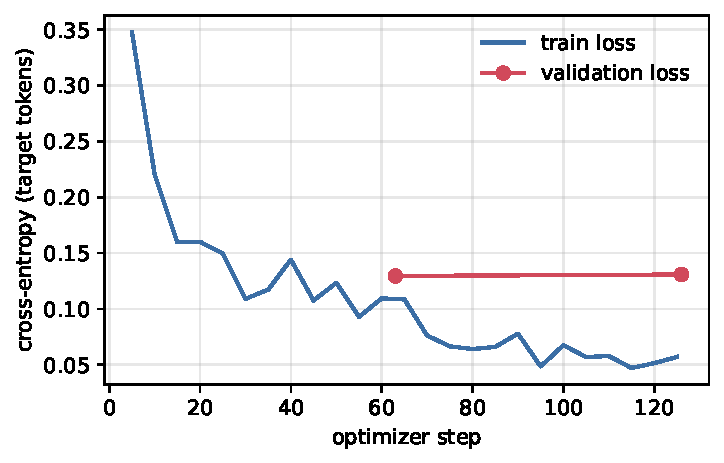
\includegraphics[width=0.88\columnwidth]{figures/training_curve_lora_qwen25_1p5b_v2.pdf}
\caption{Training and validation loss (target tokens only) of the class-balanced LoRA v2 run (126 optimiser steps, 16 minutes on a T4).}
\label{fig:curve}
\end{figure}

\subsection{Overall verdict}
The dataset is labelled per criterion, so the patient-level verdict is a transparent rule, not a learned output: any ``not included'' or ``excluded'' gives \emph{likely not eligible}; otherwise any ``not enough information'' or invalid output gives \emph{needs review}; otherwise \emph{likely eligible}. Absence of evidence is never turned into eligibility or ineligibility.

\subsection{KV-cached greedy decoding}
\label{sec:kv}
Both decoders call the model's forward pass directly instead of \texttt{generate()}. The \emph{reference} feeds the full sequence at every step with \texttt{use\_cache=False}, so step $t$ costs $O((L+t)^2)$ attention. The \emph{cached} decoder runs a prefill over the $L$ prompt tokens with positions $0..L-1$, storing per layer keys and values of shape $(1, 2, L, 128)$ in a \texttt{DynamicCache}. Each decode step then feeds only the newest token with \texttt{position\_ids}$=[p]$ and \texttt{cache\_position}$=[p]$, $p=L+t-1$; the layer appends one key/value pair, so the cache length grows by exactly one per step (asserted), and the single query attends to all $p+1$ cached keys.

\textbf{Positions.} RoPE rotates queries and keys by their absolute position \emph{before} caching, so cached keys never need re-rotation, but the new token must receive its true position: a unit test shows that feeding it at position 0 changes the logits. \textbf{Masking.} During prefill the causal mask hides future tokens; during decoding the one query is the last token, so every cached key is in its past and the mask reduces to an all-ones attention mask of length $p+1$. \textbf{Numerics.} With the cache, the new token's attention is a $1\times(p+1)$ product instead of one row of a $(p+1)\times(p+1)$ product. The arithmetic is the same but the kernel and reduction order differ, so fp16 logits can differ in the last bits; greedy outputs can diverge only at near-ties. \textbf{Prefix reuse.} In the application all criteria of one patient share the system prompt and the note, so we prefill the longest common token prefix once, decode each criterion from that cache, and crop the cache back to the prefix afterwards.

\subsection{Tiled online-softmax attention}
The reference computes $S=QK^\top/\sqrt{d}$ in fp32, masks future positions with $-\infty$ (bottom-right aligned, so it also covers $L_q<L_k$ during decoding), subtracts the row maximum before exponentiation and normalises. The tiled version processes $B_q$ query rows against $B_k$ keys at a time and keeps, per row, a running maximum $m$, normaliser $\ell$ and accumulator $a$. For a new score tile $s$:
\begin{equation}
\begin{aligned}
m' &= \max(m, \max_j s_j), & \alpha &= e^{m-m'}, & p_j &= e^{s_j-m'},\\
\ell &\leftarrow \alpha\,\ell + \textstyle\sum_j p_j, & a &\leftarrow \alpha\,a + p\,V_{\text{tile}}, & m &\leftarrow m',
\end{aligned}
\end{equation}
and finally $O=a/\ell$. This equals $\mathrm{softmax}(S)V$ exactly~\cite{milakov2018online,dao2022flashattention} but only a $B_q\times B_k$ tile exists at any time. Key tiles entirely in the future of a query tile are skipped, and only tiles crossing the diagonal are masked. A context manager routes every attention call of the Qwen2 model through this function, so the full network can run on it.

\subsection{Greedy speculative decoding}
Algorithm~\ref{alg:spec} gives our implementation. The target cache always holds the committed sequence minus its last token. The draft model catches up on all committed tokens it has not seen in one forward pass, then proposes $k$ tokens; the proposals stay on the GPU and are copied once. The target scores \([S_{-1}, d_1..d_k]\) in a single forward pass; its argmax at those $k+1$ positions are exactly the tokens plain greedy decoding would choose, because of the causal mask. The longest matching prefix ($n$ tokens) is accepted plus one target token: the correction if $n<k$, a free bonus token otherwise. Both caches are then cropped to the part that is still valid. The prompt-lookup drafter~\cite{saxena2023prompt} replaces the draft model: it finds the most recent earlier occurrence of the last 3, 2 or 1 committed tokens and proposes the $k$ tokens that followed.

\textbf{Cost model.} With per-token acceptance $\alpha$, the expected tokens per iteration are $E=(1-\alpha^{k+1})/(1-\alpha)$. Measuring the draft step cost $c$ and the cost $v_k$ of verifying $k+1$ tokens, both relative to one target decode step, the predicted speedup is
\begin{equation}
\text{speedup} \approx \frac{E(\alpha,k)}{v_k + k\,c}.
\label{eq:cost}
\end{equation}

\begin{algorithm}[t]
\caption{Greedy speculative decoding with cache rollback}
\label{alg:spec}
\footnotesize
\begin{algorithmic}[1]
\Require target $T$, drafter $D$, prompt $x$, draft length $k$
\State $S \gets x$;\; $S.\mathrm{append}(\arg\max T(x))$ \Comment{prefill $T$}
\While{not done}
  \State $d_{1..k} \gets D.\mathrm{propose}(S, k)$ \Comment{draft model or prompt lookup}
  \State $t_{1..k+1} \gets \arg\max T([S_{-1}, d_1..d_k])$ \Comment{one target pass}
  \State $n \gets$ largest $i$ with $d_{1..i}=t_{1..i}$
  \State $S.\mathrm{extend}(d_{1..n}, t_{n+1})$ \Comment{accept + correct/bonus}
  \State $T.\mathrm{cache.crop}(|S|-1)$;\; $D.\mathrm{cache.crop}(\text{valid prefix})$
\EndWhile
\end{algorithmic}
\end{algorithm}

\subsection{Application}
Fig.~\ref{fig:arch} shows the system. A FastAPI server loads the base model and the v2 adapter from the HuggingFace Hub in a background thread and serves a single-page interface. The user pastes a note (free text is split into sentences; numbered notes keep their numbering) and criteria under ``Inclusion/Exclusion Criteria'' headings, or loads a demo or validation case. Each criterion is shown with its label, cited sentence numbers and quoted evidence; clicking it highlights the evidence in the note. The overall verdict, warnings (truncation, invalid output, non-existent sentence IDs), per-criterion latency and the decoder used are displayed. Reports export as JSON, Markdown or printable HTML with the model, adapter, decoder and timestamp. Input errors return HTTP~400 with a readable message, a model that is still loading returns 503, and a ``compare decoders'' action runs one criterion through the no-cache, KV-cache and speculative decoders live. A Benchmarks tab renders the experiment logs of this paper.

\begin{figure*}[t]
\centering
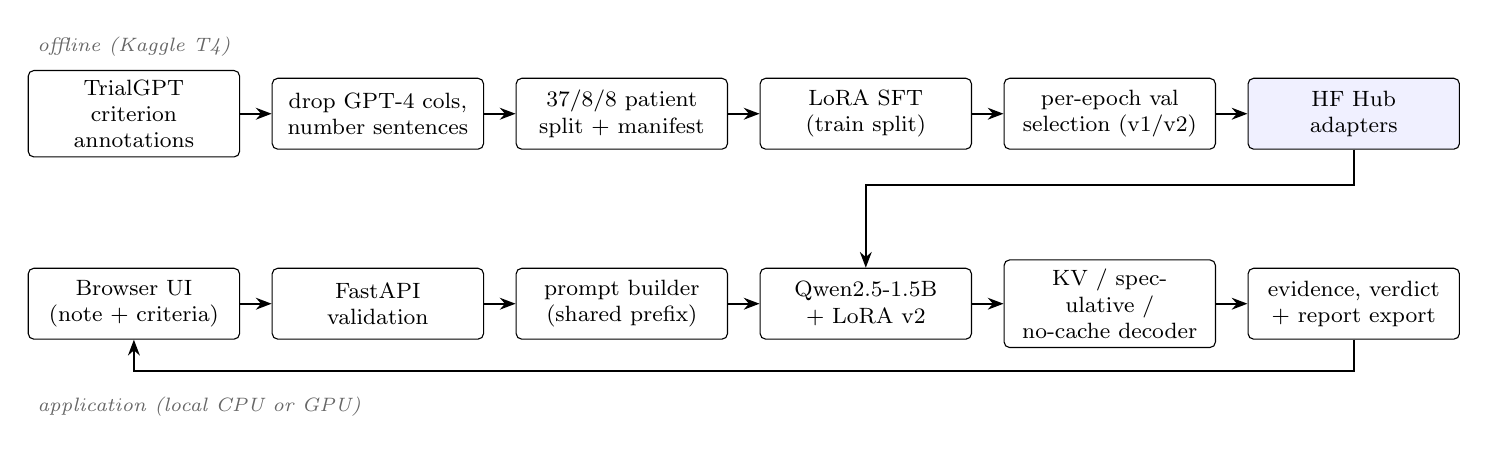
\begin{tikzpicture}[
  box/.style={draw, rounded corners=2pt, align=center, font=\footnotesize, minimum height=9mm, text width=24.5mm, fill=white},
  hub/.style={box, fill=blue!6},
  arr/.style={-{Stealth[length=2mm]}, thick},
  lab/.style={font=\scriptsize\itshape, text=black!60}]
% training row
\node[box] (ds) {TrialGPT criterion\\annotations};
\node[box, right=4mm of ds] (clean) {drop GPT-4 cols,\\number sentences};
\node[box, right=4mm of clean] (split) {37/8/8 patient\\split + manifest};
\node[box, right=4mm of split] (sft) {LoRA SFT\\(train split)};
\node[box, right=4mm of sft] (sel) {per-epoch val\\selection (v1/v2)};
\node[hub, right=4mm of sel] (hf) {HF Hub\\adapters};
\foreach \a/\b in {ds/clean, clean/split, split/sft, sft/sel, sel/hf} \draw[arr] (\a) -- (\b);
% app row
\node[box, below=14mm of ds] (ui) {Browser UI\\(note + criteria)};
\node[box, right=4mm of ui] (api) {FastAPI\\validation};
\node[box, right=4mm of api] (prompt) {prompt builder\\(shared prefix)};
\node[box, right=4mm of prompt] (model) {Qwen2.5-1.5B\\+ LoRA v2};
\node[box, right=4mm of model] (dec) {KV / speculative /\\no-cache decoder};
\node[box, right=4mm of dec] (out) {evidence, verdict\\+ report export};
\foreach \a/\b in {ui/api, api/prompt, prompt/model, model/dec, dec/out} \draw[arr] (\a) -- (\b);
\draw[arr] (hf.south) -- ++(0,-4.5mm) -| (model.north);
\draw[arr] (out.south) -- ++(0,-4mm) -| (ui.south);
\node[lab, anchor=south west] at ($(ds.north west)+(0,0.5mm)$) {offline (Kaggle T4)};
\node[lab, anchor=north west] at ($(ui.south west)+(0,-6mm)$) {application (local CPU or GPU)};
\end{tikzpicture}
\caption{System overview. Top: data preparation and training, run on a free Kaggle T4. Bottom: the browser application, which downloads the adapter and runs the hand-written decoders.}
\label{fig:arch}
\end{figure*}

% ======================================================================
\section{Experimental Setup and Metrics}
\textbf{Hardware.} Training, evaluation and benchmarks ran on one Kaggle Tesla T4 (16\,GB, fp16; T4 has no bf16). The application was tested on the author's laptop (Intel i7-8650U, 4 cores, 16\,GB RAM, fp32 on CPU). Library versions are pinned (\texttt{transformers} 4.46.3, \texttt{peft} 0.13.2).

\textbf{Decoding.} All evaluations use deterministic greedy decoding with at most 96 new tokens. Qwen's shipped generation configuration applies a repetition penalty even when sampling is off; we discovered this when comparing \texttt{generate()} with our own decoders and re-ran every reported evaluation with the penalty disabled, so that \texttt{generate()}, the KV decoder and speculative decoding are the same algorithm. The zero-shot baseline uses the identical prompt and decoding.

\textbf{Classification metrics.} Accuracy, macro-F1, per-class precision/recall/F1 and confusion matrices, overall and separately for inclusion and exclusion criteria. Macro-F1 averages over the label classes present in the gold labels of the subset (the test split has no gold ``excluded''; a zero-support class would otherwise add a constant zero). Invalid outputs are an extra confusion-matrix column and always count as wrong.

\textbf{Evidence metrics.} For gold set $G$ and predicted set $P$ per criterion: \emph{micro} P/R/F1 pool $|G\cap P|$, $|P|$ and $|G|$ over all criteria, so criteria where both sets are empty contribute nothing. \emph{Macro} P/R/F1 average per-criterion scores with $P{=}1$ if $P{=}\emptyset{=}G$, $P{=}0$ if $P{=}\emptyset\neq G$, and symmetrically for recall, so correctly citing nothing is a perfect match and citing sentences that were not annotated is penalised. Because 70\% of test criteria have empty gold evidence, we also report macro scores over the 61 criteria with non-empty gold evidence.

\textbf{Timing.} Every benchmark has a warm-up run, \texttt{torch.cuda.synchronize()} around each timed region, three repeats per configuration (median reported) and peak memory from \texttt{torch.cuda.max\_memory\_allocated} relative to the model's resident memory.

% ======================================================================
\section{Results and Discussion}
\label{sec:results}

\subsection{Before versus after fine-tuning}
Table~\ref{tab:main} and Fig.~\ref{fig:compare} compare the same model before and after fine-tuning on the identical 206 test criteria. Zero-shot, Qwen2.5-1.5B labels most exclusion criteria ``excluded'' or ``not applicable'' and never uses ``not excluded'' or ``not enough information'' (Fig.~\ref{fig:cm}, left), giving 5.3\% exclusion accuracy. Fine-tuning fixes the label semantics: accuracy rises to 0.72--0.73. v1 and v2 have similar accuracy, but v1 predicts only three of the five test classes, so its macro-F1 is 0.465; class balancing gives v2 non-zero F1 on every present class and macro-F1 0.632, and raises exclusion macro-F1 from 0.273 to 0.490. The validation ranking (v2 0.581 $>$ v1 0.468) carries over to test, which suggests the gain is not a selection artefact, although with 7 ``not included'' and 15 ``not applicable'' test criteria per-class scores move by large steps.

\begin{table}[t]
\centering
\caption{Held-out test results (206 criteria, greedy decoding).}
\label{tab:main}
\footnotesize
\setlength{\tabcolsep}{3pt}
\begin{tabular}{lccc}
\toprule
 & Zero-shot & LoRA v1 & \textbf{LoRA v2} \\
\midrule
Accuracy & 0.170 & \textbf{0.728} & 0.718 \\
Macro-F1 & 0.156 & 0.465 & \textbf{0.632} \\
Incl.\ acc.\ / macro-F1 & 0.373 / 0.207 & 0.787 / 0.426 & 0.787 / \textbf{0.610} \\
Excl.\ acc.\ / macro-F1 & 0.053 / 0.060 & 0.695 / 0.273 & 0.679 / \textbf{0.490} \\
Invalid outputs & 0 & 0 & 0 \\
\midrule
Evidence micro P / R & 0.121 / 0.691 & 0.568 / 0.489 & 0.492 / 0.691 \\
Evidence micro F1 & 0.206 & 0.526 & \textbf{0.575} \\
Evid.\ macro F1 (all) & 0.424 & 0.806 & 0.804 \\
Evid.\ macro F1 (gold$\neq\emptyset$) & 0.319 & 0.509 & \textbf{0.617} \\
\midrule
Val.\ macro-F1 (selection) & 0.143 & 0.468 & 0.581 \\
\bottomrule
\end{tabular}
\end{table}

\begin{figure}[t]
\centering
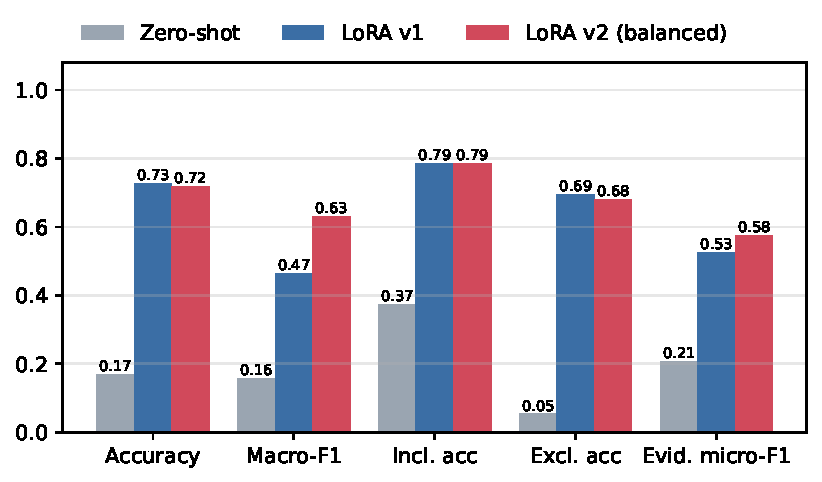
\includegraphics[width=\columnwidth]{figures/compare_baseline_test_greedy_vs_ft_v1_test_greedy_vs_ft_v2_test_greedy.pdf}
\caption{Test metrics of the same base model zero-shot, after LoRA v1 and after class-balanced LoRA v2.}
\label{fig:compare}
\end{figure}

\begin{figure}[t]
\centering
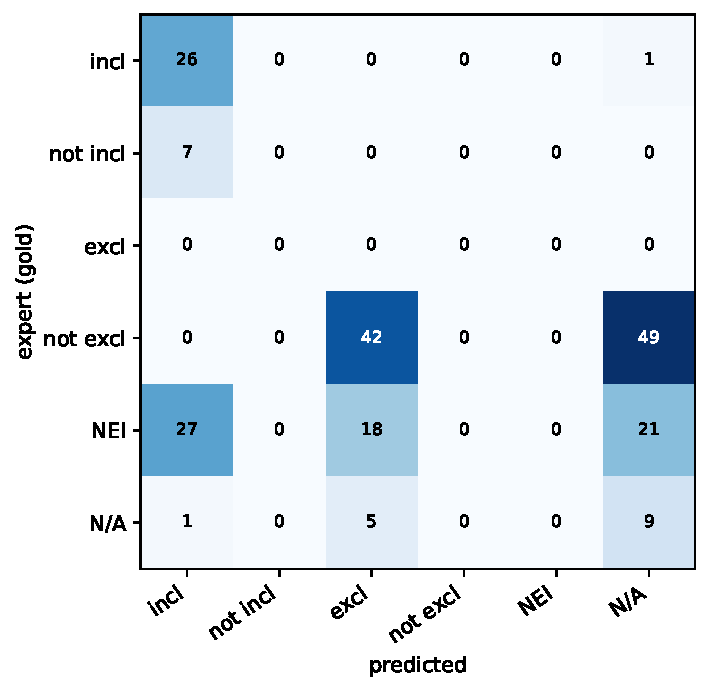
\includegraphics[width=0.49\columnwidth]{figures/cm_baseline_test_greedy_overall.pdf}\hfill
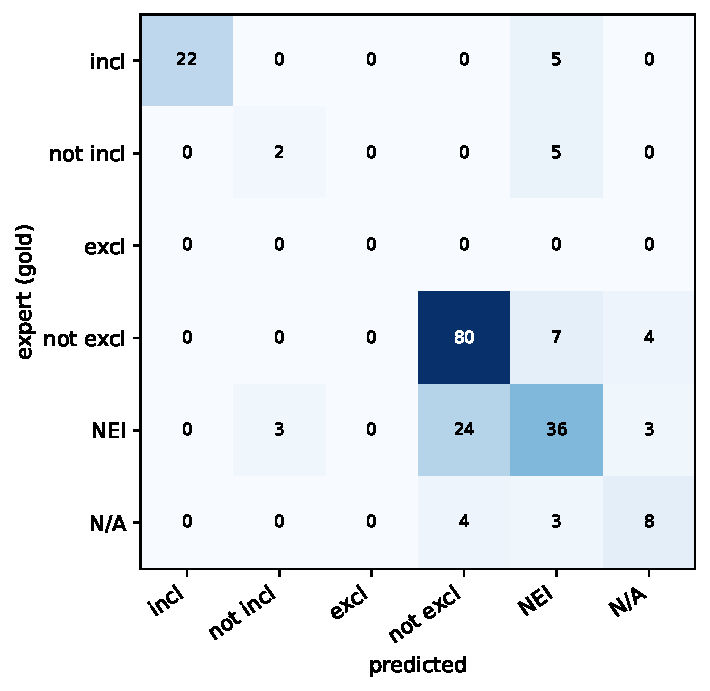
\includegraphics[width=0.49\columnwidth]{figures/cm_ft_v2_test_greedy_overall.pdf}
\caption{Test confusion matrices, zero-shot (left) and LoRA v2 (right). Rows: expert label; columns: prediction. NEI = not enough information.}
\label{fig:cm}
\end{figure}

\begin{table}[t]
\centering
\caption{Per-class test scores of LoRA v2.}
\label{tab:perclass}
\footnotesize
\begin{tabular}{lcccc}
\toprule
Class & Precision & Recall & F1 & Support \\
\midrule
included & 1.00 & 0.81 & 0.90 & 27 \\
not included & 0.40 & 0.29 & 0.33 & 7 \\
not excluded & 0.74 & 0.88 & 0.80 & 91 \\
not enough information & 0.64 & 0.55 & 0.59 & 66 \\
not applicable & 0.53 & 0.53 & 0.53 & 15 \\
excluded & -- & -- & -- & 0 \\
\bottomrule
\end{tabular}
\end{table}

Table~\ref{tab:perclass} and Fig.~\ref{fig:cm} (right) show where v2 still fails. ``included'' is almost always right when predicted (precision 1.00). The dominant error is the ``not enough information'' row: 24 of 66 such criteria are labelled ``not excluded'' and 3 ``not included''. In those 30 cases the model treats the \emph{absence} of a condition in the note as proof that the patient does not have it, which is precisely the inference the task forbids. Conversely, 20 decidable criteria are labelled ``not enough information'', the safer direction for a screener.

\textbf{Evidence.} Fine-tuning improves evidence micro-F1 from 0.206 to 0.575. Zero-shot recall looks high (0.691) only because the base model cites most of the note; precision is 0.121. v1 cited nothing for 160 of 206 criteria (higher precision, recall 0.489), while v2 recovers the zero-shot recall at four times the precision. The all-criteria macro F1 ($\approx$0.80) is inflated by the 145 criteria without gold evidence, which is why the non-empty macro F1 (0.617) is the more honest summary.

\subsection{Error analysis}
Table~\ref{tab:errors} lists ten distinct test errors of v2, taken from the automatically categorised error report (\url{results/ft_v2_test_greedy/error_analysis.md}) together with the cited sentences.

\begin{table*}[t]
\centering
\caption{Representative test errors of LoRA v2 (annotation ID, criterion, expert vs.\ model label and evidence) and their likely cause.}
\label{tab:errors}
\footnotesize
\setlength{\tabcolsep}{3pt}
\begin{tabular}{@{}p{0.6cm}p{4.4cm}p{2.4cm}p{2.4cm}p{6.9cm}@{}}
\toprule
ID & Criterion (type) & Expert & Model & Analysis \\
\midrule
174 & Previous axillary surgery (excl.) & NEI, [] & not excluded, [] & \emph{Absent evidence as proof.} The note never mentions axillary surgery; the model infers ``no'' from silence. 24 test errors follow this pattern. \\
193 & Patients were moribund (excl.) & NEI, [0--4] & not excluded, [] & \emph{Unsupported decision.} The expert cites hypotension (80/60) and tachycardia as relevant but undecidable; the model says ``not excluded'' and cites nothing. \\
162 & Open abdominal aortic aneurysm repair (incl.) & not included, [] & NEI, [0] & \emph{Over-cautious.} The patient had femoral catheterisation, not aneurysm repair; the expert concludes ``not included'' while the model asks for more information. \\
163 & Endovascular aneurysm repair (incl.) & not included, [] & NEI, [0,2] & Same patient and trial as 162: correct sentences found, but the model does not commit to the negative. \\
186 & Heart rate of at least 90/min (incl.) & included, [2] & NEI, [2] & \emph{Implicit numeric reasoning.} Sentence 2 says ``tachycardic''; the expert infers HR\,$\geq$\,90, the model finds the right sentence but wants an explicit number. \\
325 & Genetic patients (incl.) & NEI, [] & not included, [0] & \emph{Contradictory to the annotation.} A vague criterion; the model reads the demographics sentence as a negative answer. \\
322 & Pregnant women or women of childbearing age without contraception (excl.) & not excluded, [0] & not applicable, [] & \emph{Label convention.} The patient is a 48-year-old man; the expert uses ``not excluded'' (citing the sex), the model ``not applicable''. Both are defensible; the dataset is not consistent here. \\
407 & Female of child-bearing potential without contraception (excl.) & NEI, [] & not applicable, [] & A 21-year-old woman: applicability depends on contraception, which the note omits; ``not applicable'' is wrong. \\
176 & No history of central venous catheterisation (incl.) & included, [0] & included, [] & \emph{Correct label, missing evidence.} Sentence 0 (femoral arterial catheterisation) is the expert's evidence; the model cites nothing (9 such cases). \\
381 & Age $>$ 18 years (incl.) & included, [0] & included, [4] & \emph{Wrong evidence.} The age is in sentence 0; the model cites the consent sentence because the criterion mentions ``informed consent form''. \\
\bottomrule
\end{tabular}
\end{table*}

The errors fall into four groups. (1)~Treating silence as a negative finding (IDs 174, 193; 30 cases in total) is the main clinical risk because it would admit patients whose exclusion status is unknown; the rule-based verdict mitigates it only partly, since ``not excluded'' does not trigger review. (2)~Over-caution on decidable criteria (162, 163, 186) costs recall but is safe. (3)~Applicability conventions (322, 407) are partly an annotation-consistency issue. (4)~Evidence errors with correct labels (176, 381) show that the label head and the citation are not tightly coupled. None of the 206 outputs was unparseable, and no non-existent sentence ID was cited.

\subsection{KV-cached decoding}
On the 20 validation task prompts the KV decoder, the no-cache reference and HuggingFace \texttt{generate()} produced identical tokens (20/20) in both fp16 and fp32; the cache trace confirms growth from 390 to 426 positions with layer-0 keys of shape $(1,2,426,128)$. Table~\ref{tab:kv} and Fig.~\ref{fig:kv} report the length grid with EOS disabled. Prefill time is the same for both paths, as expected. The KV decoder keeps a flat 30\,tokens/s regardless of length, while the reference degrades from 24.7 to 4.3\,tokens/s because it re-encodes the whole sequence each step; the speedup grows from 1.27$\times$ to 6.90$\times$. Peak extra memory is similar (the cache costs 28\,KB/token; recomputation needs comparable activation memory). One of nine configurations diverged at generated token 150 of 256 in fp16. Re-computing that step both ways showed identical argmax tokens and a top-2 logit margin of exactly 0.0 in the reference: an exact fp16 tie, broken differently by the two kernels. In fp32 all task outputs agree.

\begin{table}[t]
\centering
\caption{No-cache vs.\ KV-cached greedy decoding (T4, fp16, median of 3).}
\label{tab:kv}
\footnotesize
\setlength{\tabcolsep}{2.6pt}
\begin{tabular}{rrrrrrrc}
\toprule
In & Out & \multicolumn{2}{c}{Prefill ms} & \multicolumn{2}{c}{Tokens/s} & Speed- & Same \\
 & & NC & KV & NC & KV & up & tokens \\
\midrule
128 & 32 & 33 & 33 & 24.7 & 31.4 & 1.27 & \checkmark \\
128 & 256 & 35 & 34 & 16.5 & 30.2 & 1.83 & @150 \\
512 & 128 & 101 & 78 & 7.8 & 30.2 & 3.87 & \checkmark \\
512 & 256 & 96 & 80 & 7.4 & 30.8 & 4.17 & \checkmark \\
1024 & 32 & 190 & 178 & 4.7 & 27.2 & 5.76 & \checkmark \\
1024 & 256 & 192 & 178 & 4.3 & 29.9 & 6.90 & \checkmark \\
\bottomrule
\end{tabular}
\end{table}

\begin{figure}[t]
\centering
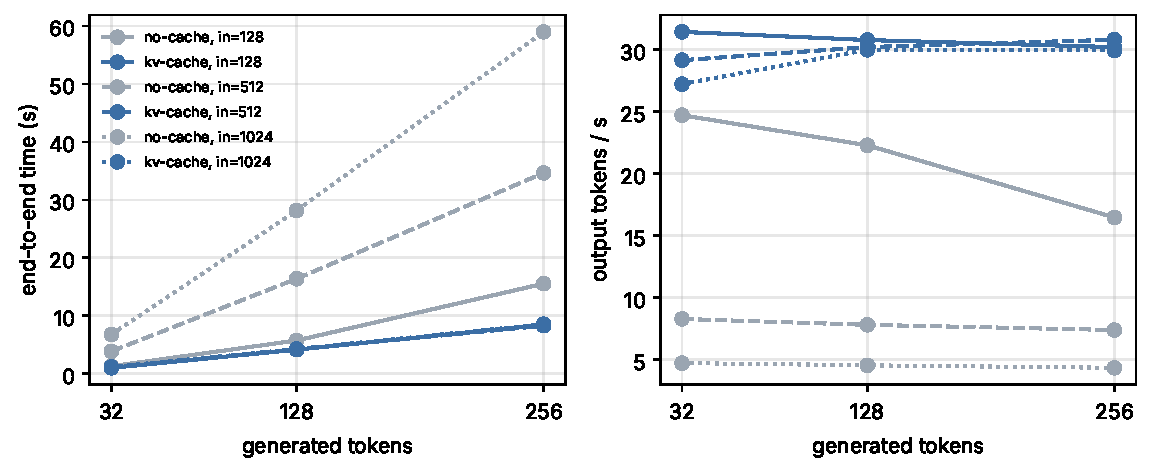
\includegraphics[width=\columnwidth]{figures/kv_cache_benchmark.pdf}
\caption{End-to-end time (left) and output tokens/s (right) of no-cache and KV-cached decoding for input lengths 128, 512 and 1\,024.}
\label{fig:kv}
\end{figure}

\subsection{Tiled attention}
Across 6 shapes (including $L_q=1<L_k$ decoding queries and lengths not divisible by the tile size), causal and non-causal masks, three tile sizes and two precisions, the tiled output matched the reference on 72/72 configurations: maximum absolute error $3.8\times10^{-6}$ (fp32) and $9.8\times10^{-4}$ (fp16), mean below $10^{-7}$. Routing all 28 layers of the fine-tuned model through it reproduced the greedy tokens of the normal model on 5/5 prompts in both precisions. Fig.~\ref{fig:attn} compares speed and memory: the reference stores the full score matrix, so its extra memory grows quadratically to 9.2\,GB at 8\,192 tokens; the tiled version needs 171\,MB (54$\times$ less), growing linearly. It is 3--4$\times$ slower than the reference because each tile is a separate Python-level matmul with its own kernel launches, whereas PyTorch's fused SDPA implements the same idea in one kernel that keeps tiles in on-chip memory, and is 18--35$\times$ faster than the reference.

\begin{figure}[t]
\centering
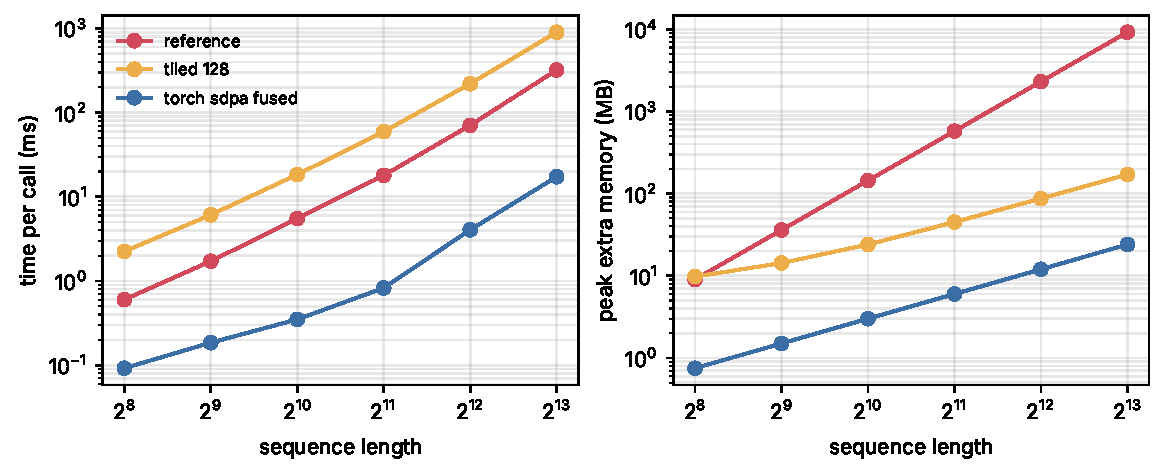
\includegraphics[width=\columnwidth]{figures/attention_benchmark.pdf}
\caption{Attention time per call (left) and peak extra memory (right) vs.\ sequence length (B=1, 12 heads, d=128, fp16, causal).}
\label{fig:attn}
\end{figure}

\subsection{Speculative decoding}
Table~\ref{tab:spec} and Fig.~\ref{fig:spec} summarise 20 task prompts (short JSON answers) and 6 note-summary prompts (longer free text). Every configuration produced exactly the target's greedy tokens (26/26). The tuned 0.5B draft is accepted 80--88\% of the time on task prompts and commits up to 4.3 tokens per target pass, yet it is \emph{slower} than plain greedy decoding (0.71--0.88$\times$). The cost model explains why: one draft step takes 25.9\,ms against 30.8\,ms for the target ($c=0.84$), because at batch size one both models are bound by per-layer kernel launches, and the 0.5B model has 24 layers to the target's 28. Verifying $k{+}1$ tokens costs only $v_k=1.10$ target steps, so with $c\approx0.85$ the denominator of Eq.~\eqref{eq:cost} grows almost as fast as the numerator. Prompt lookup has $c\approx0$, so even its low acceptance yields a real 1.16--1.19$\times$ speedup on task prompts and 1.62--2.00$\times$ on summaries, which copy long note phrases. The prediction of Eq.~\eqref{eq:cost} tracks the measurement for the draft models; for lookup it is pessimistic because 40 of its iterations had no match and cost one step instead of $v_k$. Memory grows from 3.0\,GB to 4.2\,GB with the draft model and stays at 3.1\,GB with lookup.

On the laptop CPU (Fig.~\ref{fig:app}c) the picture changes: KV caching is 6.8$\times$ faster than no-cache, but prompt lookup is 0.87$\times$, because CPU forward passes are compute bound and verifying $k{+}1$ tokens costs nearly $k{+}1$ steps, so a low acceptance rate (5 of 28 drafted tokens) does not pay off.

\begin{table}[t]
\centering
\caption{Speculative decoding vs.\ target greedy (T4, fp16). Acc.\ = draft acceptance, tok/pass = committed tokens per target forward.}
\label{tab:spec}
\footnotesize
\setlength{\tabcolsep}{2.5pt}
\begin{tabular}{llcccccc}
\toprule
Drafter & k & Same & Acc. & tok/pass & Speedup & Pred. \\
\midrule
\multicolumn{7}{l}{\emph{Task prompts (greedy: 31.0 tok/s)}} \\
lookup & 4 & 20/20 & 0.11 & 1.31 & \textbf{1.19} & 1.02 \\
base 0.5B & 4 & 20/20 & 0.55 & 2.64 & 0.66 & 0.45 \\
tuned 0.5B & 2 & 20/20 & 0.88 & 2.35 & 0.88 & 0.96 \\
tuned 0.5B & 6 & 20/20 & 0.83 & 4.33 & 0.88 & 0.70 \\
\multicolumn{7}{l}{\emph{Note summaries (greedy: 32.1 tok/s)}} \\
lookup & 8 & 6/6 & 0.19 & 2.22 & \textbf{2.00} & 1.12 \\
base 0.5B & 2 & 6/6 & 0.77 & 2.49 & 0.90 & 0.82 \\
tuned 0.5B & 2 & 6/6 & 0.78 & 2.52 & 0.90 & 0.86 \\
\bottomrule
\end{tabular}
\end{table}

\begin{figure*}[t]
\centering
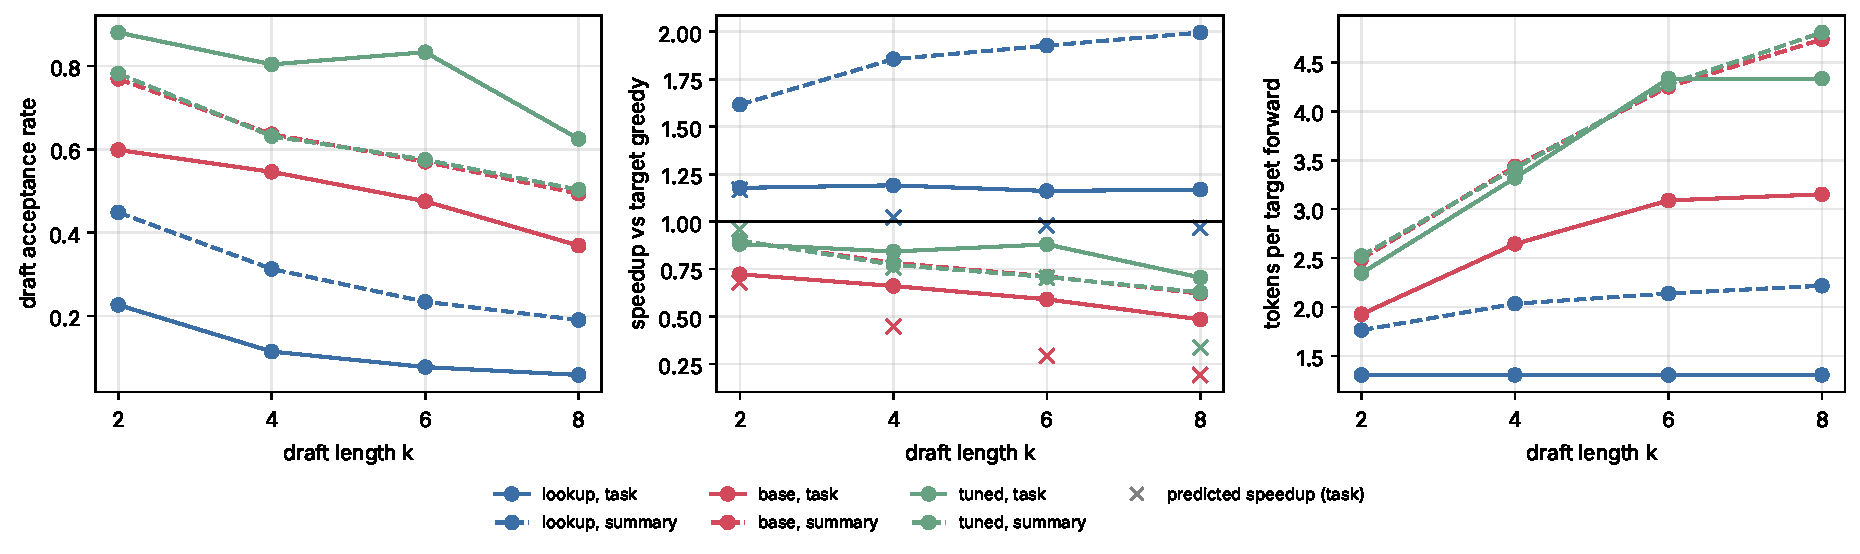
\includegraphics[width=0.92\textwidth]{figures/speculative_benchmark.pdf}
\caption{Speculative decoding vs.\ draft length $k$: acceptance (left), measured speedup with the cost-model prediction of Eq.~\eqref{eq:cost} as crosses (middle), and tokens committed per target forward pass (right).}
\label{fig:spec}
\end{figure*}

\subsection{Application}
Fig.~\ref{fig:app} shows the running application. On an unseen invented patient with six criteria it returned sensible labels with correct citations (e.g.\ ``not excluded'' for heart failure citing ``He has no history of heart failure'') and ``needs review'' because consent was not documented. On the validation patient \texttt{sigir-20141} it agreed with the expert on 17 of 21 criteria. On the laptop CPU in fp32, one criterion takes about 11--12\,s (1.3 generated tokens/s, 184 shared prompt tokens encoded once per patient); on the T4 the same evaluation runs at 6.4 criteria/s in batches.

\begin{figure*}[t]
\centering
\begin{minipage}[b]{0.49\textwidth}\centering
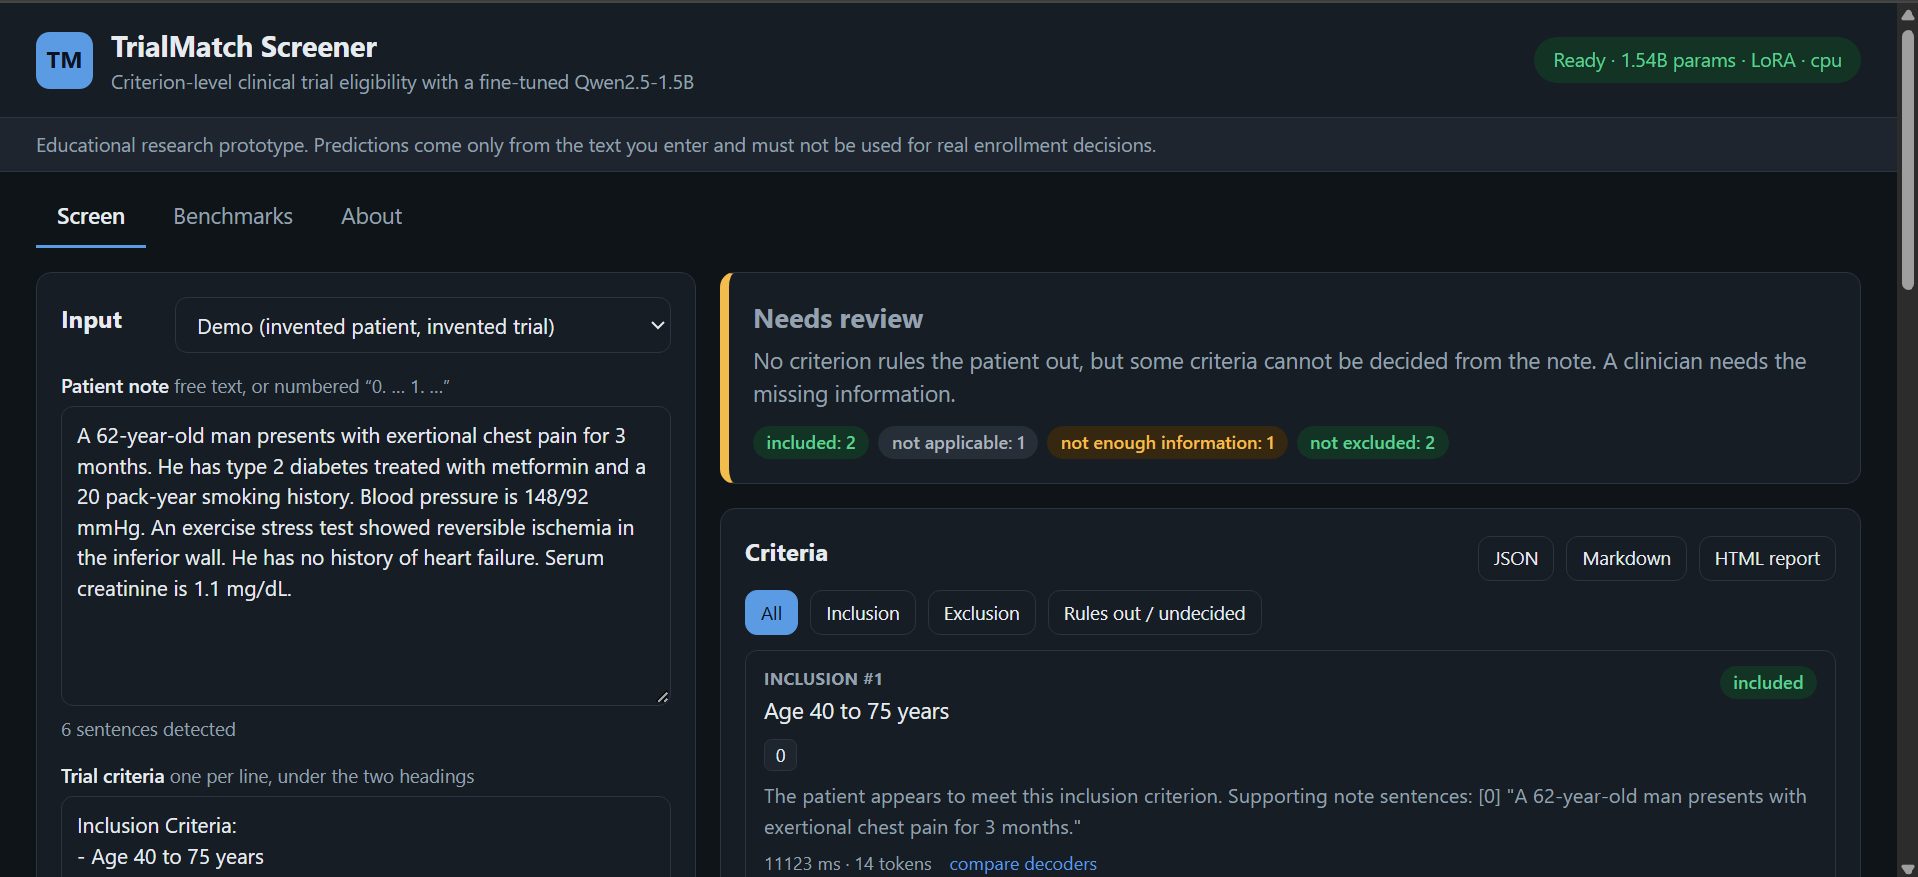
\includegraphics[width=\linewidth]{figures/app_results.png}\\[-1mm]
{\footnotesize (a) Screening result with verdict and per-criterion evidence}
\end{minipage}\hfill
\begin{minipage}[b]{0.49\textwidth}\centering
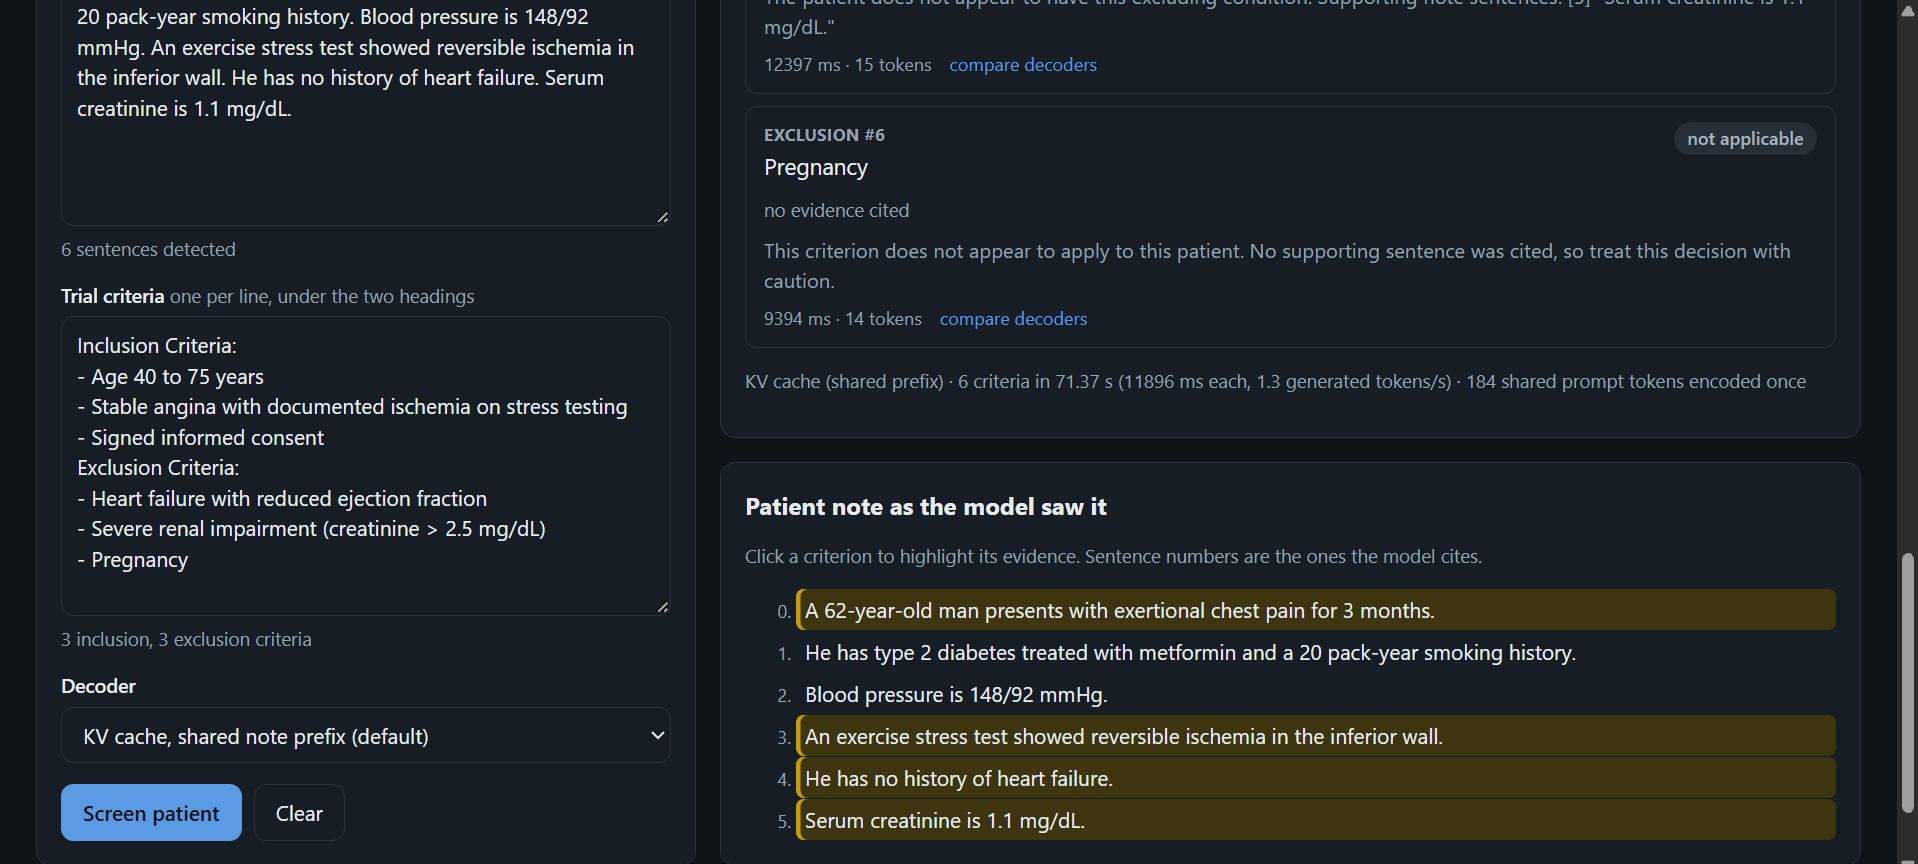
\includegraphics[width=\linewidth]{figures/app_evidence.png}\\[-1mm]
{\footnotesize (b) Evidence highlighted in the numbered note}
\end{minipage}\\[2mm]
\begin{minipage}[b]{0.40\textwidth}\centering
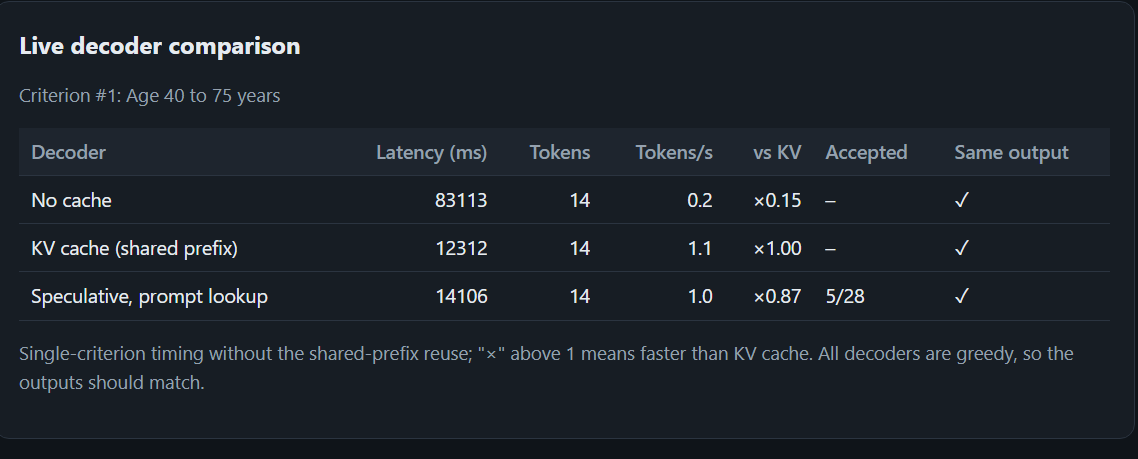
\includegraphics[width=\linewidth]{figures/app_compare.png}\\[-1mm]
{\footnotesize (c) Live decoder comparison on the laptop CPU}
\end{minipage}\hfill
\begin{minipage}[b]{0.58\textwidth}\centering

\includegraphics[width=\linewidth]{figures/app_validation.png}\\[-1mm]
{\footnotesize (d) Validation patient with agreement against expert labels}
\end{minipage}
\caption{Browser application. The Benchmarks tab (not shown) renders the tables of this section from the logged JSON results.}
\label{fig:app}
\end{figure*}

\subsection{Decisions, alternatives and difficulties}
\begin{itemize}
\item \emph{Out-of-memory at micro-batch 4} on the T4: fixed with micro-batch 1, 16-step accumulation and gradient checkpointing (peak 4.5\,GB) instead of moving to 4-bit quantisation, which would have changed the model used at inference.
\item \emph{Hidden repetition penalty} in the default generation config made \texttt{generate()} disagree with our decoders; all evaluations were redone with pure greedy decoding.
\item \emph{Minority-class collapse} of v1 led to the class-balanced v2. Oversampling was preferred over a weighted loss because it needs no change to the standard objective and is easy to audit.
\item \emph{Rejected models}: SmolLM2-1.7B (no small same-tokenizer draft, 6.9$\times$ larger KV cache, weaker zero-shot evidence) and Qwen2.5-3B (hardware limits).
\item \emph{Draft-model slowdown} motivated measuring the cost model and adding prompt lookup, the only drafter cheap enough to win on this hardware.
\item \emph{Local deployment}: Python 3.14 has no pre-built \texttt{tokenizers} wheel for the pinned version on Windows; the documented setup uses Python 3.10--3.12.
\end{itemize}

% ======================================================================
\section{Limitations}
The model is trained on 602 annotations from 37 patients and tested on 206 criteria from only 8 patients, so per-class test scores for rare labels rest on 7--15 examples and have wide uncertainty; the test split also has no ``excluded'' example. The notes are short TREC-style case reports, not real hospital records, and long records would be truncated at 3\,072 tokens. The dominant error, treating silence as a negative finding, is clinically dangerous. Explanations quote evidence but are not clinical reasoning. Speculative and attention speedups are hardware specific, and on a CPU the application needs about 11\,s per criterion. The system is an educational screening prototype and must not be used for enrollment decisions.

\section{Conclusion}
A 1.5B open-weight decoder adapted with LoRA on a free GPU raised held-out macro-F1 from 0.156 to 0.632 on criterion-level trial eligibility, kept all six expert outcome types and cited supporting sentences with 0.575 micro-F1. Hand-written KV caching, tiled online-softmax attention and speculative decoding were each verified to be exact and measured honestly: caching gave up to 6.9$\times$, tiling reduced attention memory 54$\times$ at the cost of speed, and speculative decoding was lossless but only faster with a near-free drafter, in agreement with a measured cost model. Future work should target the ``absence as proof'' errors, for example by training with explicit negative evidence and by calibrating an abstention threshold on validation data.

% ======================================================================
\section*{Reproducibility}
Code, split manifest, logs and results: \repo. Final adapter: \url{https://huggingface.co/usmanbari2005/trialmatch-qwen25-1p5b-lora-v2}; v1: \url{https://huggingface.co/usmanbari2005/trialmatch-qwen25-1p5b-lora}; draft: \url{https://huggingface.co/usmanbari2005/trialmatch-qwen25-0p5b-draft-lora}. Kaggle notebooks \texttt{01}--\texttt{04} reproduce every table; \texttt{python -m app} (or \texttt{start\_app.bat}) starts the application. Demonstration video: \videolink.

\appendix
\section*{AI-Use Statement}
Claude (Anthropic) was used as a coding and writing assistant: it drafted most of the source code (data pipeline, training and evaluation scripts, KV-cache, attention and speculative decoders, tests and the web application) and a first draft of this report from the logged results. The author ran all experiments on Kaggle and on his laptop, debugged failures (out-of-memory, Kaggle session limits, Windows setup), reviewed and tested the code (72 automated tests), checked every number in this paper against the result files, and is responsible for the submission. No AI system produced any reported result: all numbers come from executed code on the fixed split.

\begin{thebibliography}{99}
\bibitem{jin2024trialgpt} Q.~Jin, Z.~Wang, C.~S. Floudas, F.~Chen, C.~Gong, D.~Bracken-Clarke, E.~Xue, Y.~Yang, J.~Sun, and Z.~Lu, ``Matching patients to clinical trials with large language models,'' \emph{Nature Communications}, vol.~15, art.~9074, 2024.
\bibitem{koopman2016test} B.~Koopman and G.~Zuccon, ``A test collection for matching patients to clinical trials,'' in \emph{Proc. 39th Int. ACM SIGIR Conf.}, 2016, pp.~669--672.
\bibitem{vaswani2017attention} A.~Vaswani, N.~Shazeer, N.~Parmar, J.~Uszkoreit, L.~Jones, A.~N. Gomez, {\L}.~Kaiser, and I.~Polosukhin, ``Attention is all you need,'' in \emph{Advances in Neural Information Processing Systems}, 2017.
\bibitem{su2024roformer} J.~Su, M.~Ahmed, Y.~Lu, S.~Pan, W.~Bo, and Y.~Liu, ``RoFormer: Enhanced transformer with rotary position embedding,'' \emph{Neurocomputing}, vol.~568, 2024.
\bibitem{ainslie2023gqa} J.~Ainslie, J.~Lee-Thorp, M.~de~Jong, Y.~Zemlyanskiy, F.~Lebr{\'o}n, and S.~Sanghai, ``GQA: Training generalized multi-query transformer models from multi-head checkpoints,'' in \emph{Proc. EMNLP}, 2023.
\bibitem{qwen2025report} Qwen Team, ``Qwen2.5 technical report,'' arXiv:2412.15115, 2024.
\bibitem{allal2025smollm2} L.~B. Allal \emph{et~al.}, ``SmolLM2: When smol goes big --- data-centric training of a small language model,'' arXiv:2502.02737, 2025.
\bibitem{hu2022lora} E.~J. Hu, Y.~Shen, P.~Wallis, Z.~Allen-Zhu, Y.~Li, S.~Wang, L.~Wang, and W.~Chen, ``LoRA: Low-rank adaptation of large language models,'' in \emph{Proc. ICLR}, 2022.
\bibitem{pope2023efficiently} R.~Pope, S.~Douglas, A.~Chowdhery, J.~Devlin, J.~Bradbury, A.~Levskaya, J.~Heek, K.~Xiao, S.~Agrawal, and J.~Dean, ``Efficiently scaling transformer inference,'' in \emph{Proc. MLSys}, 2023.
\bibitem{kwon2023paged} W.~Kwon, Z.~Li, S.~Zhuang, Y.~Sheng, L.~Zheng, C.~H. Yu, J.~E. Gonzalez, H.~Zhang, and I.~Stoica, ``Efficient memory management for large language model serving with PagedAttention,'' in \emph{Proc. ACM SOSP}, 2023.
\bibitem{dao2022flashattention} T.~Dao, D.~Y. Fu, S.~Ermon, A.~Rudra, and C.~R{\'e}, ``FlashAttention: Fast and memory-efficient exact attention with IO-awareness,'' in \emph{Advances in Neural Information Processing Systems}, 2022.
\bibitem{milakov2018online} M.~Milakov and N.~Gimelshein, ``Online normalizer calculation for softmax,'' arXiv:1805.02867, 2018.
\bibitem{leviathan2023fast} Y.~Leviathan, M.~Kalman, and Y.~Matias, ``Fast inference from transformers via speculative decoding,'' in \emph{Proc. ICML}, 2023.
\bibitem{chen2023accelerating} C.~Chen, S.~Borgeaud, G.~Irving, J.-B. Lespiau, L.~Sifre, and J.~Jumper, ``Accelerating large language model decoding with speculative sampling,'' arXiv:2302.01318, 2023.
\bibitem{saxena2023prompt} A.~Saxena, ``Prompt lookup decoding,'' GitHub repository, 2023. [Online]. Available: \url{https://github.com/apoorvumang/prompt-lookup-decoding}
\end{thebibliography}

\end{document}
